\section{Future Research}
\label{sec:future-research}

After running the experiments and analyzing the results, we have identified some areas of (potential) improvement in the system. In this section we will discuss some of these areas.

\paragraph{Experimenting with Knowledge Depth}
In Section \ref{sssec:knowledge-depth} the concept of knowledge depth was mentioned. As this research kept it at a constant value of 1, it would be interesting to see how this system would perform with different values. This could be done by running the experiments again, but with different values for the knowledge depth. This would give a better understanding of how the knowledge depth affects the performance of the system.

\paragraph{Updating Risk Rules}
Another area for further research is the risk rules. As mentioned in Section \ref{sssec:risk-rules}, the risk rules are quite simple. It would be interesting to see how the system would perform with more complex risk rules. This could be done by running the experiments again, but with more complex risk rules. This would give a better understanding of how the risk rules affect the performance of the system. 

\paragraph{Simplifying the Attackgraph}
During the implementation and experimentation some back-and-forth discussions were held about the risk reports that were sent during an auction. The risk reports contain a subsection of the entire attackgraph a node calculated, containing only the nodes that are part of the risk path the auction tries to mitigate. This subsection would contain all risk edges between the nodes, including their probabilities (See figure \ref{fig:riskreport-a}). This would result in a large amount of data being sent during an auction. 

\begin{figure}[H]
    \centering
    \begin{subfigure}[b]{0.4\textwidth}
        \centering
        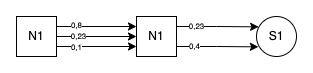
\includegraphics[width=\textwidth]{_content/riskreport-future-research-a.png}
        \caption{Full risk report with all edges.}
        \label{fig:riskreport-a}
    \end{subfigure}
    \hspace{0.5cm}
    \begin{subfigure}[b]{0.4\textwidth}
        \centering
        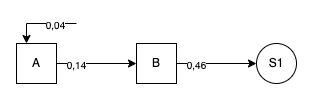
\includegraphics[width=\textwidth]{_content/riskreport-future-research-b.png}
        \caption{Merged risk report with only one edge.}
        \label{fig:riskreport-b}
    \end{subfigure}
    \caption{Two different methods of dealing with risk reports, where on the left all risk edges are present and no information is lost. On the right all risk edges between nodes have been merged into a single edge, resulting in a smaller amount of data being sent.}
\end{figure}


An alternative to sending all edges, was to merge the probabilities of all the edges between two nodes into a single edge (See figure \ref{fig:riskreport-b}). This merging could be done similar to the logic that is used when calculating the risk damage value, for example $p = \prod_{k=1}^{R} (1 - p_{k})$ where $R$ is the risk edges between the nodes, and $p_{k}$ is the probability for an edge. 
This would result in a smaller amount of data being sent during an auction. However, this would also result in a loss of information. Since there are no actual messages sent over the network in the experiments, the amount of data that was sent was not a bottleneck, so the decision was made to send all edges of the subgraph. However, if this system were to be implemented in a real-world scenario, the amount of data sent could be a bottleneck. In that case, it would be interesting to see how the system would perform with the alternative risk report.

\paragraph{Cost and Time}
The current implementation of the system does not take the cost and time of a proposal into account. This means that the system will always choose the proposal with the lowest risk damage value, regardless of the cost and time of the proposal. We acknowledge that this is not a realistic scenario, as the cost and time of a proposal are important in real-life situations. Budgets and time are often critical factors when making decisions about what mitigation strategy to implement, as sometimes the cost of a proposal is too high, or the time it takes to implement is too long. Allowing the system to perform Cost-Benefit Analysis (CBA) such as suggested by Butler \cite{butler2002security} would be a good addition to the system. As a future research the system's \code{ProposalSelector} could be improved to do Cost-Benefit Analysis. We would expect to see a significant change in the speed/efficiency at which the damage of the system reduces, as a budget would potentially filter the candidate-proposals. However, by collecting metrics of the costs of the proposals, we might see a more cost-effective solution that could still reduce the damage of the system.

\add{Mention the effects of compromised agents and the impact}
